\begin{section}{The Delivery Man}
  To understand our solution and the algorithms that we have forcefully gladly chosen to implement, we must first explore the problem and study what it is that we are trying to accomplish. This is done first by describing a problem setting, describing the situation and what we will try to accomplish.
  Secondly, we introduce a mathematical formalisation of the problem in terms of a game The game provides a rigurous \textbf{abstraction} which will greatly simplify our theoretical analysis of the problem and the $A^*$-algorithm used to solve it. This section is based on \cite{run} and \cite{lab}.
  
  \begin{subsection}{Problem Setting}
    From this point on, you are a delivery boy for the company ``Planet Express'', a man who has been sent to a small, two-dimensional city with a well-known rectangular street layout. The first task, which you have already accomplished, is to travel to intersection $(x, y)$ and get into a car. In the car, you have found a note which contains a list of pick-up and delivery points (all at intersections), $(x_{p_i}, y_{p_i}, x_{d_i}, y_{d_i})$, for $i\in \{1,2,3,4, 5\}$. 

    Your mission, according to the note, is to pick up and deliver all the packages in some order, without ever having more than one package in your car at a given time. It is also company policy, apparently, according to the note, that if you are at a pick-up point $(x_{p_i}, y_{p_i})$ you have to pick the package up. Similarly, the note clearly states that if company policy is every broken, dire consequences will be faced by someone. By you.
    
    You discover that the car doors are locked, and you note that the back side of the note says that the doors may be open once your work has been done. By you. Now, it seems that your company is completely unconcerned about your work-load, survival or well-being. However, \textbf{for you it is important to minimize time spent working}.

    Fortunately, the city's traffic control office provides continuous, up-to-date information about traffic load for each road-segment at each moment in time. So at each intersection, if you can develop some algorithm that is fast enough at computing, you will be able to determine the most optimal route at each intersection. Or, if you find it appropriate, you could wait a while at the intersection. It is up to you, it's not as if Hubert J. Farnsworth, the not so benevolent dictator of ``Planet Express'' has any idea of what is going on.
  \end{subsection}

  \begin{subsection}{Game Construction}
    We begin by introducing a planar graph $G$ that can be visualized as a rectangular grid, which gives an intuition of how the game looks and provide the game board. We assume that we have been given a tuple $(m, n)$ of integers $m \geq 1, n \geq 1$ which define the vertical and horizontal \textbf{dimensions} of the game, respectively.
    
    \begin{subsubsection}{The Game Graph}
    Consider $[m]\times [n]$, where $[k] = \{1, ..., k\}$ for positive $k$. Furthermore, we denote the \textbf{horizontal edges} between node $(i, j)$ and $(i, j+1)$ in $[m] \times [n]$ by $h_{i,j}$. Similarly, we denote the \textbf{vertical edges} between node $(i, j)$ and $(i+1, j)$ in $[m] \times [n]$ by $v_{i,j}$. Finally, we also define $0_{i,j}$ as ``the edge'' from $(i,j)$ to $(i,j)$. 

    Note that the $m\cdot (n-1)$ horizontal, and $(m-1)\cdot n$ vertical edges in our construction can be drawn such that the graph, lest the loops $0_{i,j}$, consists of an exterior rectangle within which there are $m-2$ horizontal and $n-2$ vertical lines, with nodes $(i, j)$ in the intersection of the $i$:th horizontal and $j$:the vertical line. See figure \ref{fig:grid}.

      \begin{figure}[H]
        \label{fig:grid}
        \centering
        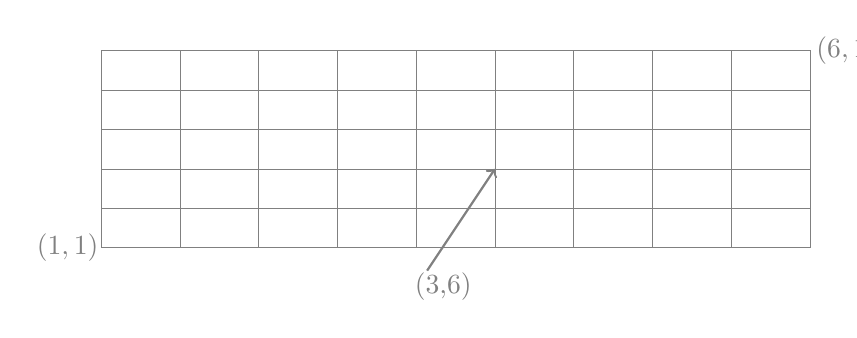
\begin{tikzpicture}[gray,very thin]
          \draw (0,0) -- (9,0) -- (9,2.5) -- (0,2.5) -- (0,0);
          \node[text width=1] at (-0.8,0) {$(1,1)$};
          \node[text width=1] at (9.1, 2.5) {$(6,10)$};
          \draw (1,0) -- (1,2.5);
          \draw (2,0) -- (2,2.5);
          \draw (3,0) -- (3,2.5);
          \draw (4,0) -- (4,2.5);
          \draw (5,0) -- (5,2.5);
          \draw (6,0) -- (6,2.5);
          \draw (7,0) -- (7,2.5);
          \draw (8,0) -- (8,2.5);
          \draw (0,0.5) -- (9,0.5);
          \draw (0,1) -- (9,1);
          \draw (0,1.5) -- (9,1.5);
          \draw (0,2) -- (9,2);
          \node[text width=1] (fourfive) at (4,-0.5) {(3,6)};
          \draw[->, thick] (fourfive) -- (5,1);
        \end{tikzpicture}
        \caption{Graph $G$ with dimension (6,10), edges $0_{i,j}$ not drawn for clarity.}
      \end{figure}
      
    Mathematically, we let our graph $G$ have underlying vertices $V = [m] \times [n]$, and edge-set $E$ defined by the vertical and horizontal edges $h_{i,j}$ and $v_{i,j}$ as above, as well as $0_{i,j}$. That is $E$ is formally defined by the binary relation
    \begin{equation}
      \begin{split}
      E = \{((i, j), (i, j+1)) &= h_{i,j}, 1 \leq i \leq m, 1 \leq j \leq (n-1)\}
      \\ \cup \{((i, j), (i+1, j)) &= v_{i,j}, 1 \leq i \leq (m-1), 1 \leq j \leq n \}
      \\ \cup \{((i, j), (i, j)) &= 0_{i,j}, 1 \leq i \leq m, 1 \leq j \leq n \}.
      \end{split}
    \end{equation}

    Note that we have made formal sense of the notion of nodes $(i, j)$, horizontal edges $h_{i,j}$ and vertical edges $v_{i,j}$ in terms of a graph. Similarly, it makes sense to talk about \textit{the grid of $G$}.

    \end{subsubsection}
    
    \begin{subsubsection}{The Game}
      TODO: Checka att det jag skriver överrensstämmer med hur programmet fungerar.

       Suppose that we are given the game dimension $(m, n)$ and have a graph $G$ constructed as above. Furthermore, we are given a \textbf{starting point} $(x, y)\in V$, and a finite set of \textbf{packages} $P = \{(p_i, d_i), i \in [k]\} \subseteq V\times V$. Furthermore, we play the game as follows:
      \begin{itemize}

        \item \textit{Objective}: For starting point $(x,y)$, and packages $P$, your objective is to pick up each package $(p,d)\in P$ at pick-up point $p$ and deliver it to corresponding delivery point $d$ by following the horizontal and vertical edges in $E$. That is, the \textbf{objective} is to deliver all the packages.

        \item \textit{Rules}:
          The game is played in turns. Each turn $t$, you may take one of the following \textbf{actions} $A = \{a_1, ..., a_5 \}$:
          \begin{enumerate}
          \item \textit{Up}: Move from node $(i, j)$ to node $(i+1, j)$.
          \item \textit{Down}: Move from node $(i, j)$ to node $(i-1, j)$.
          \item \textit{Left}: Move from node $(i, j)$ to node $(i, j-1)$.
          \item \textit{Right}: Move from node $(i, j)$ to node $(i, j+1)$.
          \item \textit{Stay}: Stay at node $(i, j)$.
          \end{enumerate}
          
          If an action is \textbf{valid}, you start turn $t+1$ on the indicated to-node. An action is \textbf{invalid} if the indicated to-node does not exists, in which case the action is taken to be $a_5$ and you remain at the same node at turn $t+1$.\\
          \textbf{Turns} are enumerated by increasing integers starting with $t = 1$. 

        \item \textit{Mechanics}:
          The mechanics are partly governed by the constraints.
          \begin{itemize}
          \item You \textbf{arrive} at a node $(i, j)$ at turn $t$ if the action you took at turn $t-1$ makes your position for turn $t$ node $(i, j)$.
            
          \item A package $(p, d)$ is \textbf{picked up} in turn $t$ if you arrive at node $p = (i, j)$ at turn $t$, and you do not hold a package when you arrive.

          \item You \textbf{hold} a package $p$ in turn $t$ if you've picked up $p$ in turn $t' \leq t$ and have not yet delivered the package. 

          \item A package $(p, d)$ is \textbf{delivered} in turn $t$ if you arrive at node $d = (i, j)$ at turn $t$ and you hold the package $(p, d)$.  

          \end{itemize}
          
        \item \textit{Mechanical constraints}:
          \begin{itemize}
          \item You do not pick up a package in the same turn that you deliver a package.
          \item You do not pick up a package at the start of the game (turn $t = 1$).
          \item You can only hold one package at a time.
          \item You can never change packages.
          \item If you can pick up a package, you will.
          \item If you can deliver a package, you will.
          \item You can not pick up the same package twice.
          \end{itemize}
      \end{itemize}

      Furthermore, during each turn $t$, we have access to the following functions, which may depend both on the current turn $t$ or turns $t' \neq t$:
      \begin{itemize}
      \item A status function $s_t: P \rightarrow \{0,1,2 \}$, which determines one of the following statuses for each package on your delivery route:
        \begin{itemize}
        \item $s_t(p) = 0$ indicates that you have not picked up nor delivered the package.
        \item $s_t(p) = 1$ indicates that you have picked up (and consequently currently hold) the package.
          
        \item $s_t(p) = 2$ indicates that you have delivered package $p$.
        \end{itemize}

      \item A function $me: \mathbb{N} \rightarrow M\times N \cup \{\emptyset \}$, where $me(t')$ gives your location $(i, j)$ for your current turn or turns $t' \leq t$, or $\emptyset$ otherwise.

      \item A cost function $c_t: E \rightarrow \mathbb{N}$ associated with each edge, and $c(0_{i,j}) = 0$. For example, if it is turn $3$ and we want to know the cost of the horizontal edge $h_{2,3}$ going from vertice $(2, 3)$ to vertice $(2, 4)$ at turn $3$, we call $c_3(h_{2,3})$.

      \item An edge function $e: A\times V \rightarrow E$ such that $e(a, (i,j)) = ((i, j),(i',j'))$ where $(i', j')$ is the node that results from taking action $a$ in position $(i,j)$ if the action is valid, and just $(i, j)$ otherwise.

      \item Past action function $\texttt{past}: \mathbb{N} \rightarrow A\cup \{\emptyset\}$, where $\texttt{past}(t')$ gives us the action $a_{i_{t'}}$ taken at time $t' < t$ or $\texttt{past}(t') = \emptyset$ for $t' \geq t$.
      \end{itemize}

      We only have access to functions $s_t, c_t$ for our current turn $t$ or $t' < t$, and never for $t' > t$. That is, we can not see into the future.
      
      A game \textbf{strategy} is \textit{how} and \textit{in what order} to deliver each package.

      A \textbf{solution} is a \textit{finite} sequence of actions $A_{seq} = (a_{i_1}, ..., a_{i_T})$, given in a \textit{finite} amount of time, associated with each turn that delivers all packages.

      Your \textbf{score} is determined by
      \begin{equation*}
        \sum_{t = 1}^T c_t(e(a_{i_t}, me(t)))
      \end{equation*}      

      \begin{paragraph}{Notes about the game 1.}
        By the mechanics, you may ``accidentally'' pick up a package that you would not want to pick up just yet, which may constrain \textit{how} you chose your route to the next pick-up destination. If the pick-up points for two packages $p_1, p_2$ coincide, there is no way to determine which will be picked up.
      \end{paragraph}

      \begin{paragraph}{Notes about the game 2.}
        For starting point $(x, y)$, you have not arrived at point $(x,y)$ at turn $t=1$. To arrive at that point, you have to chose action $a_5$ and arrive at $(x, y)$ at turn $t=2$, or arrive at a later turn.
      \end{paragraph}

      \begin{paragraph}{Notes about the game 3.}
        For a given edge $x\in E$, $c_t(x), c_{t'}(x)$ gives potentially different values when $t \neq t'$.
      \end{paragraph}

    \end{subsubsection}
    
    \begin{subsubsection}{Performance metric}
      The game above seems trivial if we were uninterrested in the score. For example, a finite solution for $k$ packages would be to just traverse the entire grid $2k$ times, which would take a maximum of $mn(2k+1)$ steps\footnote{To \textit{arrive} in a corner may take a maximum of $mn$ steps, which ensures that traversing the entire graph twice delivers at least one package.}.

      Our interresting in the game is to minimize the cost of edge traversals while providing a tractable answer to the game. That is, \textbf{we search for a solution $A_{seq}$ that is solution to the game above, and which minimizes the total score}. 
    \end{subsubsection}

    TODO icke-negativa edges är ett krav för A*?
  \end{subsection}

  

\end{section}
